%!TEX root = ../report.tex
\section{Problem Definition}
% Give a precise formulation of the problem you will be addressing
Since the fluids are simulated using SPH, the fluid is discretized in different particles.
A scene containing a fluid, simulated by SPH, can be seen in figure \ref{fig:sph}.
Since this ``fluid'' does not look like a fluid that can be found in nature, a visualization technique has to be applied.

\begin{figure}[!th]
\hrule
\begin{center}
\vspace*{2ex}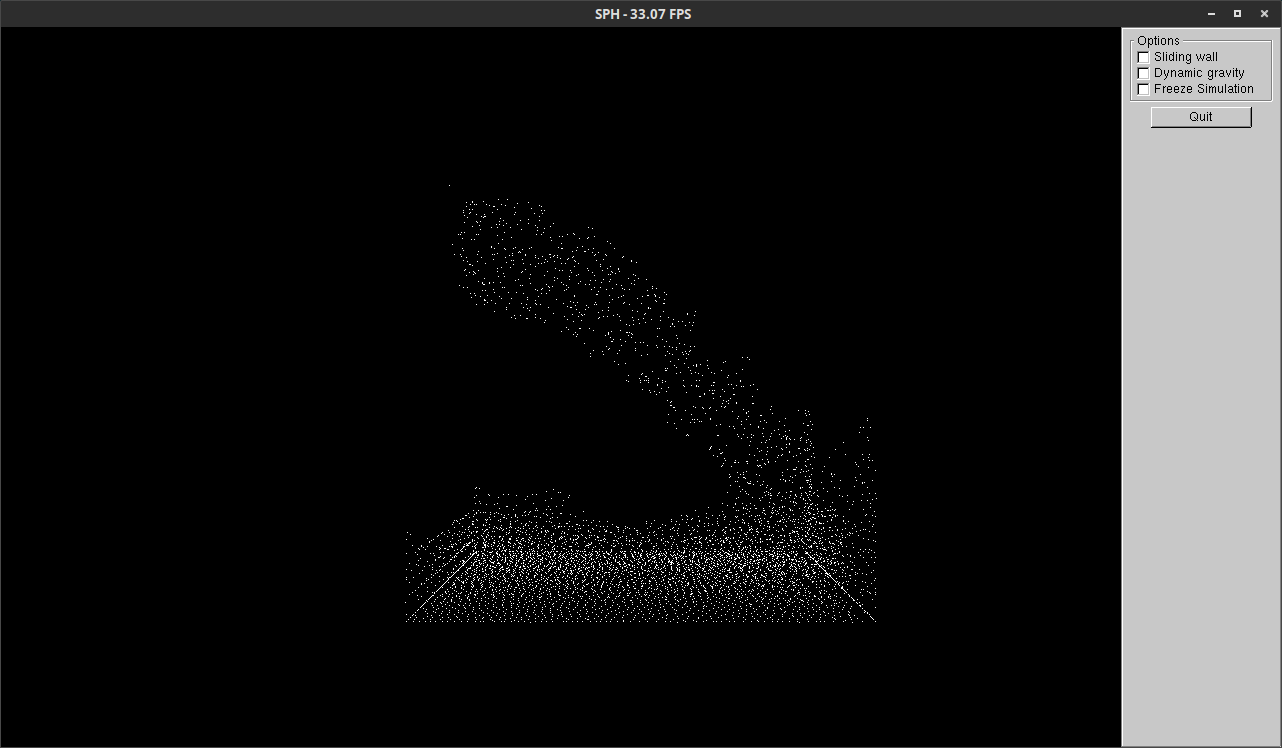
\includegraphics[width=0.48\textwidth,clip=true,trim=10cm 3cm 10cm 3cm]{pictures/sph.png}
\end{center}
\caption{SPH simulation}
\label{fig:sph} 
\vspace*{2ex}
\hrule
\end{figure}

It is our goal to create a nature-like rendering of fluids that can be rendered in real-time, in order to use it in games, for example.
It is also desirable to make sure that the rendering can be customized according to the requirements of users.
For example, fluids can have different kind of thicknesses, or the quality of the rendering can be altered in order to keep the rendering in real-time.

It is also import to distinct what makes a rendering realistic and in real-time. 
We define real-time to be a simulation that is smooth, stutter-free and runs in about the same as the real world.
In practice, this is not always feasible and therefore we define a simulation to be real-time if it produces at least 20 frames per second.

A nature-like visualization of a fluid is a tangible concept as humans have a clear vision of what is a realistic visualization and what is not, but it is not quite as easy to formally define.

There are several components that contribute to a realistic visualization of a fluid.
In order to be realistic a fluid surface needs to be smooth. That is, there are no sharp discontinuities between particles.

Moreover, the surface needs to be imperfect. This may sound counter-intuitive as it contradicts with the point that a surface needs to be smooth, but it turns out that in nature a fluid surface is rarely perfectly smooth due to wind and other natural effects.

Finally, a fluid should also act as a fluid in a simulation. This means that object attributes as color should be attenuated as that object is submerged in the fluid and the fluid should produce foam if it is mixed with gases in large quantities. 

The combinations of these components are what can make a fluid surface visualization realistic and it these components we seek.
\subsection{Related work}
Various methods are developed that try to achieve a nature-like rendering of fluid.
Some of these techniques require to use a mesh, which is not desirable.
Other techniques have the drawback that they can not be rendered in real-time.

\cite{zhang2008adaptive} developed a method that makes use of point-based rendering, therefore a grid is unnecessary.
However, a drawback of this method is that it results in unreasonably thick surfaces.
